\documentclass[class=article, crop=false]{standalone}
\usepackage{standalone}
\usepackage{pageslts}
\usepackage{hyperref}
\usepackage{booktabs}
\usepackage{listings}
\usepackage[latin1]{inputenc}
\usepackage{tikz}
\usetikzlibrary{shapes,arrows}
\usepackage[utf8]{inputenc}

% Language setting
% Replace `english' with e.g. `spanish' to change the document language
\usepackage[english]{babel}

% Set page size and margins
% Replace `letterpaper' with `a4paper' for UK/EU standard size
\usepackage[letterpaper,top=2cm,bottom=2cm,left=3cm,right=3cm,marginparwidth=1.75cm]{geometry}

% Useful packages
\usepackage{amsmath}
\usepackage{graphicx}
\usepackage[colorlinks=true, allcolors=blue]{hyperref}

% packages for math modes
\usepackage{amsmath,amssymb,mathtools,bm} % define this before the line numbering.
\usepackage[digitsep]{siunitx}

% package for tables
\usepackage{booktabs}
% package for codes
\usepackage{ctex}
\usepackage{float}
\usepackage{listings}

\lstset{
    basicstyle          =   \sffamily,
    keywordstyle        =   \bfseries,
    commentstyle        =   \rmfamily\itshape,
    stringstyle         =   \ttfamily,
    flexiblecolumns,
    numbers             =   left,
    showspaces          =   false,
    numberstyle         =   \zihao{-5}\ttfamily,
    showstringspaces    =   false,
    captionpos          =   t,
    frame               =   lrtb,
}

\lstdefinestyle{Matlab}{
    language        =   Matlab,
    basicstyle      =   \zihao{-5}\ttfamily,
    numberstyle     =   \zihao{-5}\ttfamily,
    keywordstyle    =   \color{blue},
    %keywordstyle    =   [1] \color{violet},
    keywordstyle    =   [2] \color{magenta},
    stringstyle     =   \color{orange},
    commentstyle    =   \color{teal}\ttfamily,
    breaklines      =   true,
    columns         =   fixed,
    basewidth       =   0.5em,
}

\renewcommand{\lstlistingname}{Code}% Listing -> Algorithm

% package for appendices
\usepackage[toc, page]{appendix}

%%%%%%%%%%%%%%%%%%%%%%%%%%%%%%%%%%%%%%%%%%%%%%%%%%%%%%%%%%%%%%%%%%%%%%
\title{The report the Inertial Navigation Exercise 1}
\author{Shiqi Jiang}

\begin{document}
\maketitle

\begin{abstract}
This report is a description of Inertial Navigation (LUH) Exercise 1, which covers mathematical theories applied in solving the tasks in the exercise and scientific computation via coding, as well as visualising the results. The data set used in the code comes from the file \verb|ex01_10042889.mat|, and the results are stored in the file \verb|ex01_10042889.csv|. All of the codes for this exercise are included in the appendix.
\end{abstract}

\section{Introduction}

In inertial navigation, measurement of specific forces and turn rates are integrated to estimate position, velocity and attitude of an object. In order to integrate those values, integration constants are needed, which are gained with GNSS for position and velocity for instants. The attitude of the IMU can be provided by an initial alignment. To transform the specific forces measured in the body-frame into an arbitrary target-system, the attitude of the object has to be provided at any time. Ultimately, the task the attitude update is solved by the gyroscope and its turn rate measurement, which is used to compute the rotation matrix of the b-frame to the n-frame.\cite{1}

\section{Part A: Initial Aligment and orientation representation}

\subsection{Task 1: Roll-, pitch and yaw angles, DCM}
To find initial orientation for attitude computation, the computation of Euler angles and the Direction Cosine Matrix (DCM) is extremely significant. Inclination in b-frame is commonly calculated by the following formulas:

\begin{center}
    \begin{subequations}
    \begin{align}
        &\phi_0 = \operatorname{atan2}{(-\overline{f}_{ib,y}^b, -\overline{f}_{ib,z}^b)} \label{1a} \\
        &\theta_0 = \arctan{(\frac{\overline{f}_{ib,x}^b}{\sqrt{(\overline{f}_{ib,y}^b)^2 + (\overline{f}_{ib,z}^b)^2}})} \label{1b} \\
        &\psi_0 = \arctan{(\frac{\overline{\omega}_{ib,y}^b)}{\overline{\omega}_{ib,x}^b)})} \label{1c}
    \end{align}
    \end{subequations}
\end{center}

And in MATLAB for rotation Matrix/DCM can be calculated by the following three methods:

\begin{itemize}
    \item Calculate the three basic rotation matrices before synthesising
    
    \begin{center}
        \begin{subequations}
        \begin{align}
            &C_3(\psi) =
            \begin{pmatrix}
            \cos{(\psi)} & \sin{(\psi)} & 0 \\
            -\sin{(\psi)} & \cos{(\psi)} & 0 \\
            0 & 0 & 1
            \end{pmatrix} \\
            &C_2(\theta) =
            \begin{pmatrix}
            \cos{(\theta)} & 0 & -\sin{(\theta)} \\
            0 & 1 & 0 \\
            \sin{(\theta)} & 0 & \cos{(\theta)}
            \end{pmatrix} \\
            &C_1(\phi) =
            \begin{pmatrix}
            1 & 0 & 0 \\
            0 & \cos{(\phi)} & \sin{(\phi)} \\
            0 & -\sin{(\phi)} & \cos{(\phi)}
            \end{pmatrix} \\
            &C_n^b = C_1(\phi) \cdot C_2(\theta) \cdot C_3(\psi)
        \end{align}
        \end{subequations}
    \end{center}

    \item Calculating each cell in rotation matrix directly
    
        \begin{center}
            \begin{subequations}
            \begin{align}
                &C_{11} = \cos{(\theta)} \cdot \cos{(\psi)} \\
                &C_{12} = -\cos{(\theta)} \cdot \sin{(\psi)} + \sin{(\phi)} \cdot \sin{(\theta)} \cdot \cos{(\psi)} \\
                &C_{13} = \sin{(\theta)} \cdot \sin{(\psi)} + \cos{(\phi)} \cdot \sin{(\theta)} \cdot \cos{(\psi)} \\
                &C_{21} = \cos{(\theta)} \cdot \sin{(\psi)} \\
                &C_{22} = \cos{(\theta)} \cdot \cos{(\psi)} + \sin{(\phi)} \cdot \sin{(\theta)} \cdot \sin{(\psi)} \\
                &C_{23} = -\sin{(\theta)} \cdot \cos{(\psi)} + \cos{(\phi)} \cdot \sin{(\theta)} \cdot \sin{(\psi)} \\
                &C_{31} = -\sin{(\theta)} \\
                &C_{32} = \sin{(\phi)} \cdot \cos{(\theta)} \\
                &C_{33} = \cos{(\phi)} \cdot \cos{(\theta)} \\
                &C_n^b = {C_b^n}^T =
                \begin{pmatrix}
                C_{11} & C_{12} & C_{13} \\
                C_{21} & C_{22} & C_{23} \\
                C_{31} & C_{32} & C_{33} \\
                \end{pmatrix}^T
            \end{align}
            \end{subequations}
        \end{center}
    
    \item The function \verb|angle2dcm()|
\end{itemize}

With coding, the result of computation is finally as follows

\begin{itemize}
    \item Initial roll angle [deg]: 0.14986
    \item Initial pitch angle [deg]: : 0.0011211
    \item Initial yaw angle [deg]: : -40.3596
    \item DCM via all 3 methods:
    \begin{equation}
        C_n^b =
        \begin{pmatrix}
            0.7620 & -0.6476 & -0.0000 \\
            0.6476 & 0.7620 & 0.0026 \\
            -0.0017 & -0.0020 & 1.0000 \\
        \end{pmatrix}.\notag
    \end{equation}
\end{itemize}

\subsection{Task 2: Gravity and Earth rotation}
To estimate the local gravity $g$, as well as the Earth rotation rate $\omega_e$ with the given data, it is necessary to apply the following formulas:

\begin{itemize}
    \item The local gravity
    \begin{equation}
        g = f(\overline{f}_x, \overline{f}_y, \overline{f}_z)
    \end{equation}
    \item The Earth rotation rate
    \begin{equation}
        \omega_e = f(\overline{\omega}_x, \overline{\omega}_y, \overline{\omega}_z)
    \end{equation}
\end{itemize}

The corresponding function in MATLAB code is \verb|norm()|. And note that the unit here is "rad/s", converting the unit to "deg/h" is necessary if to make it more readable.

The acceleration the Earth gravity and the Earth rotation rate, which are commonly used in calculation, are 9.81 $\mathrm{m/s^2}$ and 15 $\mathrm{deg/h}$, respectively. And the data computed by coding are $g = 9.8391 \ \mathrm{m/s^2}$ and $\omega_e = 87.031 \ \mathrm{deg/h}$. The reason for the difference between here and the former may be the latitude or altitude at which the sensor is located on Earth.

\subsection{Task 3: Rotation vector and Quaternion}
By the rotation axis/angle representation or by the corresponding quaternion are two methods to express the initial orientation. The required parameters can be calculated using the following equations:

\begin{itemize}
    \item Rotation vector
    \begin{equation}
        u_{nb} = \frac{\vec{\delta}}{|\vec{\delta}|} \quad \text{ with } \vec{\delta} =
        \begin{pmatrix}
            C_{32}-C_{23}\\
            C_{13}-C_{31}\\
            C_{21}-C_{12}
        \end{pmatrix}
    \end{equation}
    \item Rotation axis/angle
        \begin{subequations}
        \begin{align}
            &\operatorname{trace}(C_n^b) = 2 \cos{(\delta)} + 1\\
            &\sin^2{(\delta)} + \cos^2{(\delta)} = 1 \Rightarrow \sin{(\delta)} = \sqrt{1 - \cos^2{(\delta)}}
        \end{align}
        \end{subequations}
    \item Quaternion
        \begin{subequations}
        \begin{align}
            &q = \begin{pmatrix} a\\ b\\ c\\ d \end{pmatrix} =
            \begin{pmatrix}
                \cos{(\frac{\alpha}{2})}\\
                \sin{(\frac{\alpha}{2})} \omega
            \end{pmatrix} \\
            &a = \frac{1}{2} \sqrt{1 + \operatorname{trace}(C_n^b)}\\
            &\begin{pmatrix} b \\ c \\ d \end{pmatrix} = \frac{1}{4a} \begin{pmatrix}
            C_{32}-C_{23}\\
            C_{13}-C_{31}\\
            C_{21}-C_{12}
            \end{pmatrix}
        \end{align}
        \end{subequations}
\end{itemize}

After computation, the initial orientation expressed by the rotation axis as

\begin{equation}
    \begin{pmatrix}
        -0.0036\\
        0.0013\\
        1.0000
    \end{pmatrix} \notag
\end{equation}

\noindent with the angle $\delta$ as 0.70441 Rad, and also could be expressed by the corresponding quaternion as

\begin{equation}
    \begin{pmatrix}
        0.9386\\
        -0.0012\\
        0.0004\\
        0.3450
    \end{pmatrix}. \notag
\end{equation}

If the approximated yaw angle is to be read via the rotation axis/angle representation, the magnitude of this vector approximates the yaw angle, provided that the axis of rotation is nearly vertical (Z-axis). if representation via the Quaternion, the yaw angle can be extracted from a quaternion using the following formula:

\begin{center}
\begin{equation}
    \mathrm{Yaw} = \operatorname{atan2}{(2*(a*d + b*c), 1 - 2*(c^2 + d^2))}.
\end{equation}
\end{center}

\section{Part B: Attitude Update}

\subsection{Task 4: Direct calculation of the direction cosine matrix}
Added some pre-conditions in Part B:

\begin{center}
    \begin{subequations}
    \begin{align}
    &g^n = [0, 0, -g],\\
    &\omega_{ie}^n = \omega_e \cdot [\cos{(\varphi), 0, -\sin{(\varphi)}}]^T \text{ with } \varphi = 52.385828^{\circ}.
    \end{align}
    \end{subequations}
\end{center}

The local gravity $g = 9.8391 \ \mathrm{m/s^2}$ and the Earth's rotation rate $\omega_e = 4.2194e-04 \ \mathrm{Rad/s}$ can be calculated in the same way as in Task 2, and the specific values can be calculated by substituting them into the above formulas. The DCM can then be calculated directly by substituting the following formula:

\begin{center}
\begin{equation}
    [f_{ib}^b, \omega_{ib}^b, f_{ib}^b \times \omega_{ib}^b] = C_n^b \cdot [g^n, \omega_{ie}^n, g^n \times \omega_{ie}^n] \Rightarrow \mathrm{L} = C_n^b \cdot \mathrm{R}.
\end{equation}
\end{center}

\noindent The final result is calculated as

\begin{center}
\begin{equation}
    C_n^b = \mathrm{L} \cdot \mathrm{R}^{-1} = [f_{ib}^b, \omega_{ib}^b, f_{ib}^b \times \omega_{ib}^b] \cdot [g^n, \omega_{ie}^n, g^n \times \omega_{ie}^n]^{-1} =
    \begin{bmatrix}
    1.1198 & -0.9497 & -0.0000\\
    0.9550 & 1.1198 & 0.0026\\
    2.0224 & -0.0029 & 1.0000
    \end{bmatrix}. \notag
\end{equation}
\end{center}

Evidently it is not the same as the result the computation in Part A (see Section 2.1, P. 3). To check out whether the DCM is orthogonal or not, multiply it with its own transpose matrix, if the result is identity matrix then it is orthogonal, otherwise it is not. By computation as

\begin{center}
\begin{equation}
    C_n^b \cdot {C_n^b}^T =
    \begin{bmatrix}
    2.1559 & 0.0059 & 2.2673\\
    0.0059 & 2.1660 & 1.9308\\
    2.2673 & 1.9308 & 5.0900
    \end{bmatrix} \neq I \notag
\end{equation}
\end{center}

\noindent can be learnt that the new DCM is not orthogonal , therefore re-orthogonalisation is necessary. Using approximation by minimising the track could do re-orthogonalisation the new DCM, and the corresponding mathematical formula\cite{2} is as follows:

\begin{center}
\begin{equation}
    \mathrm{\overline{A} = A(A^T A)^{-\frac{1}{2}}}.
\end{equation} \label{12}
\end{center}

\noindent Substituting $C_n^b$ into $A$ calculated the re-orthogonalised DCM

\begin{center}
\begin{equation}
    C_n^b \Leftarrow C_n^b \cdot ({C_n^b}^T \cdot C_n^b)^{-\frac{1}{2}} =
    \begin{bmatrix}
    0.6616 & -0.5105 & -0.5493\\
    0.3786 & 0.8597 & -0.3430\\
    0.6473 & 0.0189 & 0.7620
    \end{bmatrix}. \notag
\end{equation}
\end{center}

However, this method is not globally applicable. For example, when an aircraft is located at the South Pole or the North Pole, at which point it is more complexly affected by the gravitational field and magnetic field from the Earth.

\subsection{Task 5: Attitude Update}

The closed-form solution will be applied in the last task. The closed-form solution assumes that IMU is at rest or in uniform motion. It is assumed that IMU is not moving in n-frame. Finally, the Euler angles over time are plotted and the final orientation of the sensor will be estimated.\cite{1}

Due to the static IMU, the transportation rate is ignored. IMU measures the sum of all rotations $\omega_{nb}^b$ in b-frame:

\begin{center}
\begin{equation}
    \omega_{nb}^b = \omega_{ib}^b - C_n^b \omega_{in}^n = \omega_{ib}^b - C_n^b \cdot (\omega_{en}^n + \omega_{ie}^n) = \omega_{ib}^b - C_n^b \cdot \omega_{ie}^n.
\end{equation}
\end{center}

After transform corrections solve the matrix differential equation (See Formula 14) in update-step.

\begin{center}
\begin{equation}
    \dot{C}_b^n = C_b^n \Omega_{nb}^b.
\end{equation}
\end{center}

The solution is as follows (The time interval $\Delta t$ in IMU data set is equal to 0.01):

\begin{center}
    \begin{subequations}
    \begin{align}
    &C_b^n(t+\Delta t) = C_b^n(t) \cdot [I + \frac{\sin{\delta}}{\delta}(\delta \times) + \frac{1-\cos{\delta}}{\delta^2} (\delta \times)^2]\\
    &\text{ with } \delta = ||\vec{\delta}||, \delta = \omega_{nb}^b \Delta t \\
    &(t+\Delta t) =
    \begin{bmatrix}
    0 & -\delta_3 & \delta_2\\
    \delta_3 & 0 & -\delta_1\\
    -\delta_2 & 0 & \delta_1
    \end{bmatrix}
    \end{align}
    \end{subequations}
\end{center}

After the corresponding computation, the new rotation matrix has to be re-orthogonalized, and ultimately the Euler angles can be calculated using Equation 3 (see Section 2.1, P. 2) and the inverse trigonometric functions:

\begin{center}
    \begin{subequations}
    \begin{align}
    &\Phi = \operatorname{atan2}(\frac{C_{32}}{C_{33}})\\
    &\Theta = \arcsin{(-C_{31})}\\
    &\Psi = \operatorname{atan2}(\frac{C_{21}}{C_{11}}).
    \end{align}
    \end{subequations}
\end{center}

The final Euler angles can be computed as respectively:

\begin{itemize}
    \item The estimated final Roll Angle $\Phi$ is $-24.2316 ^\circ$,
    \item The estimated final Pitch Angle $\Theta$ is $33.322 ^\circ$,
    \item The estimated final Yaw Angle $\Psi$ is $-37.6537 ^\circ$.
\end{itemize}

\noindent And an image of the Euler angles over time is shown below (See Figure 1).

\begin{figure}
\centering
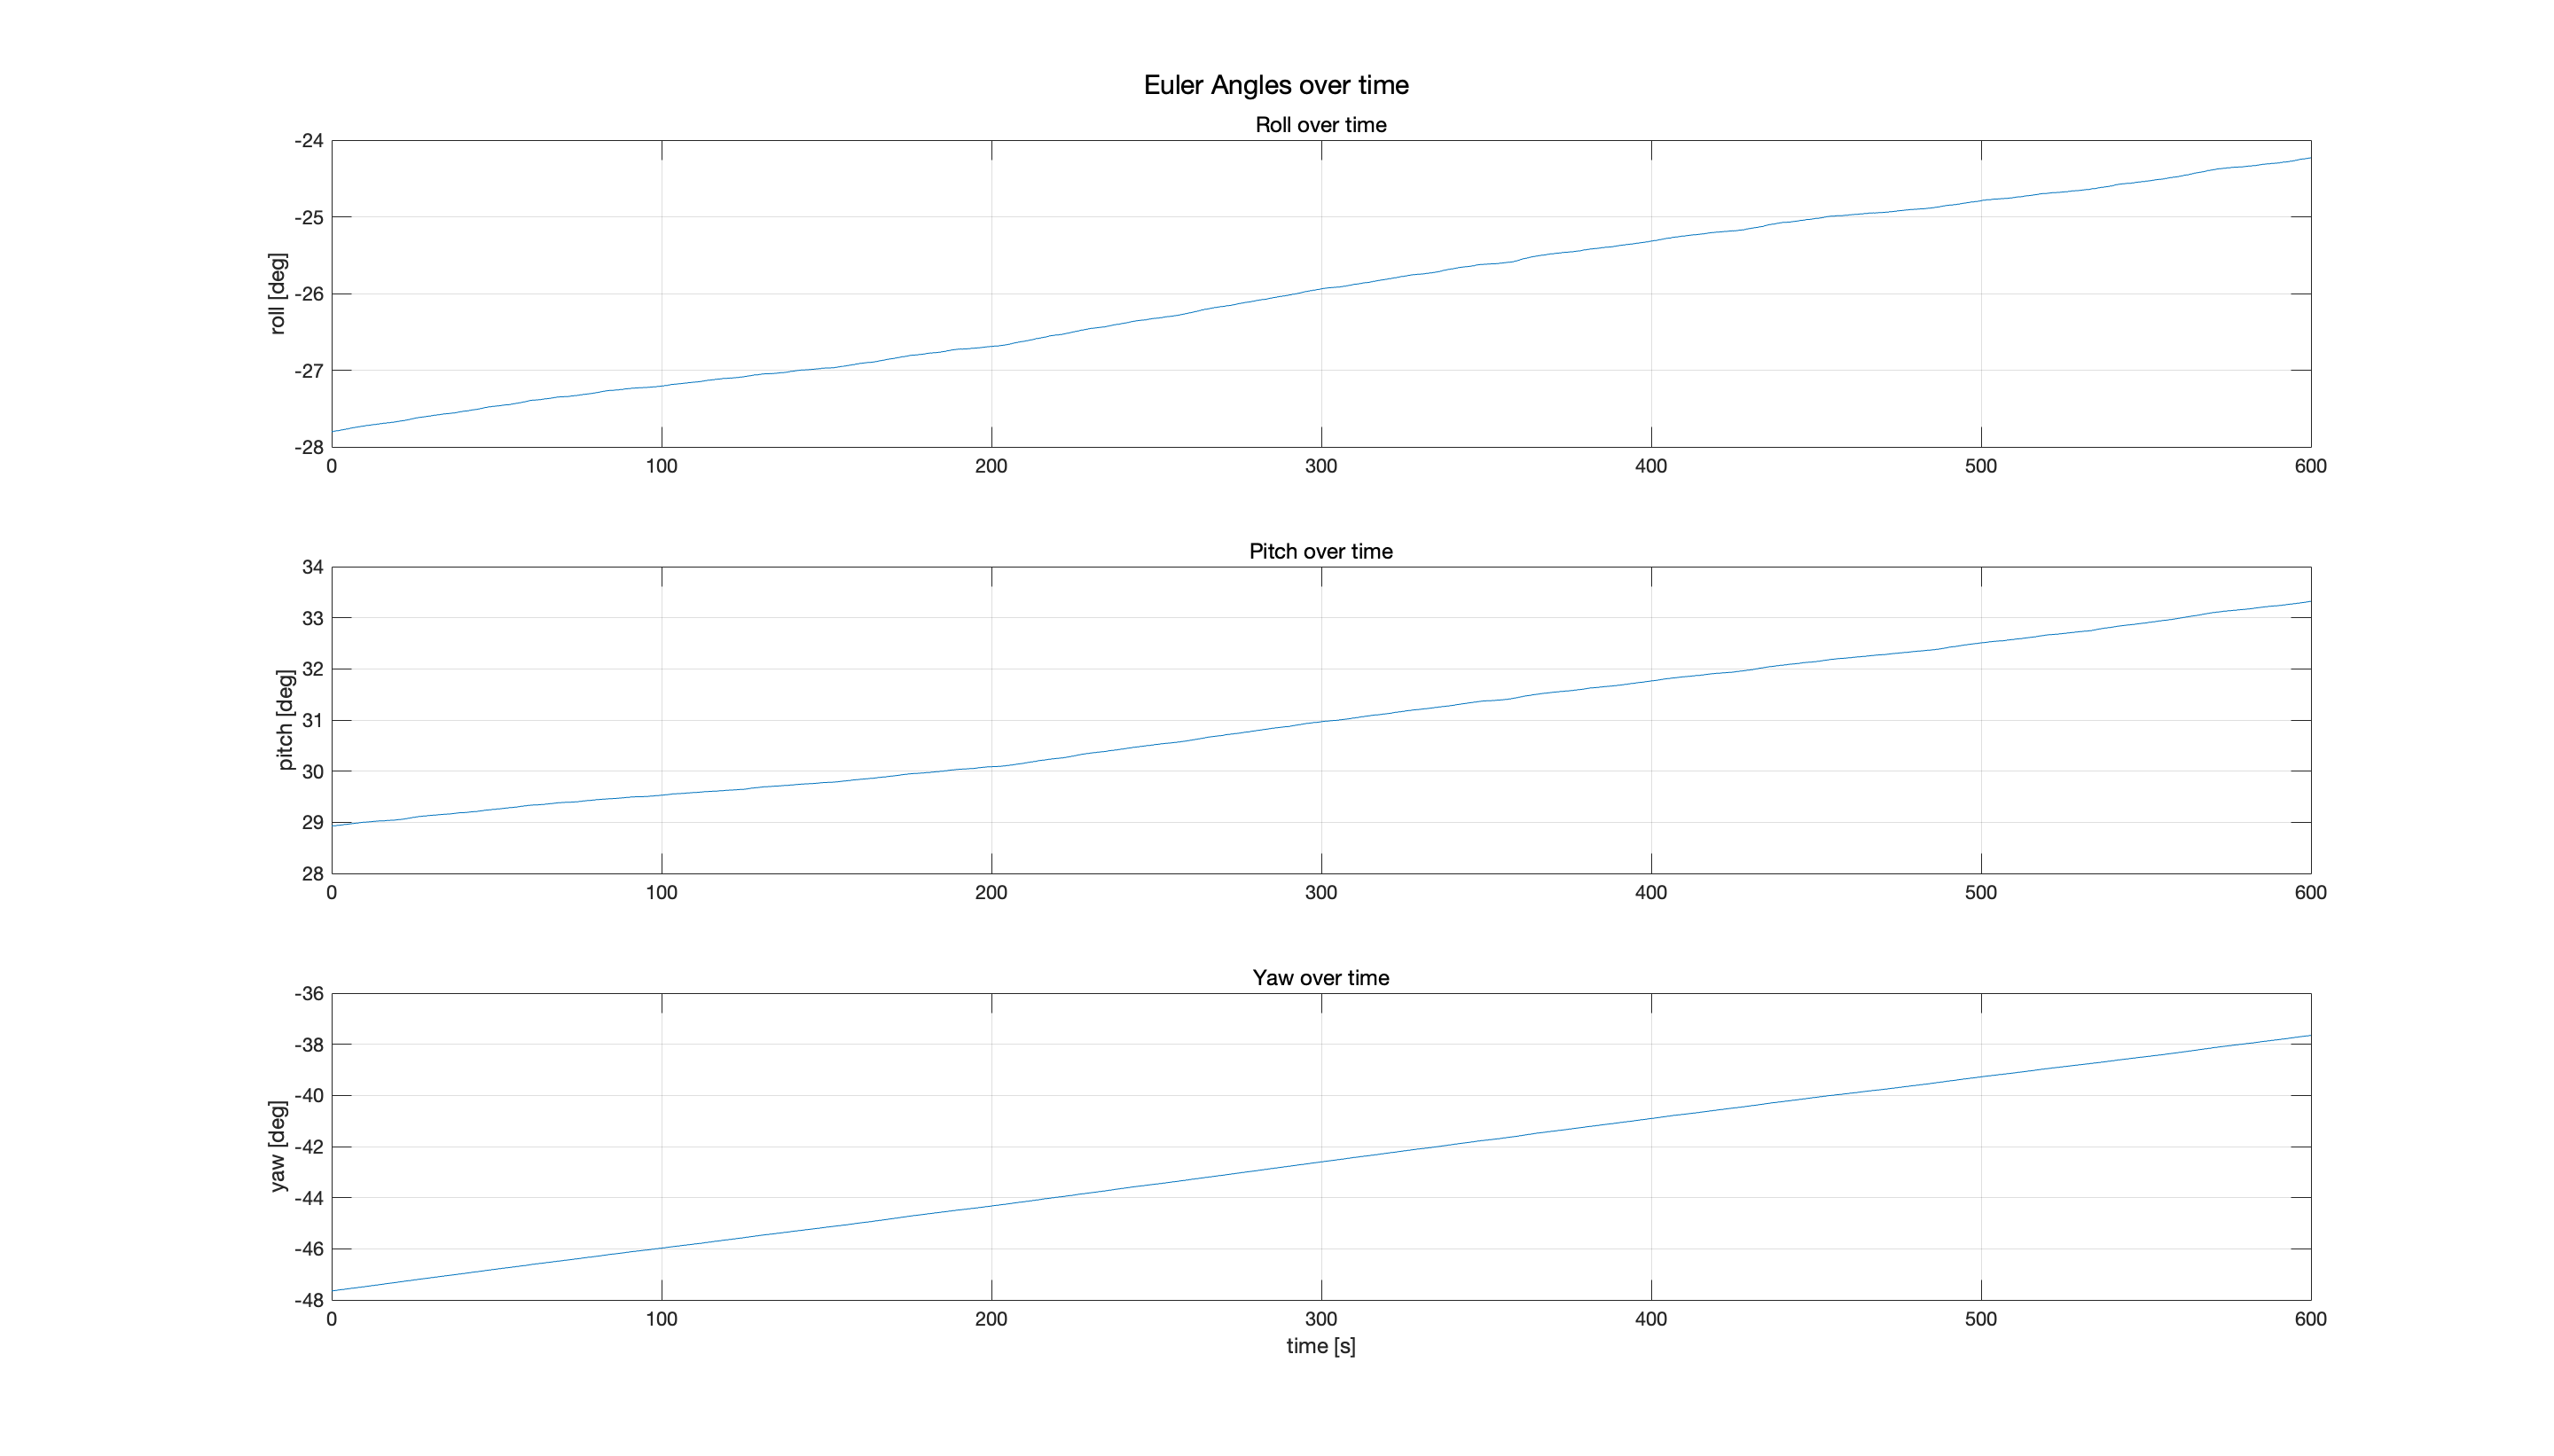
\includegraphics[width=1\textwidth]{ex01b_task5.png}
\caption{\label{fig:task5}Plot the evolution of the three Euler-angles over time.}
\end{figure}

In a static IMU the Euler angle still changes over time, possible factors are internal (e.g. noise in sensors).

\section{Conclusion}
The rotational axis should always be orthogonal to each other, as insufficient orthogonality of the axis can induce cross-coupling.

To analyze the sensor errors and calibrate them is always necessary. In tasks the Planet Rotation Rate is calculated to be 87.0310 $\mathrm{[deg/h]}$, which is impossible on Earth, and if this data is not measured near a neutron star, then a high probability that it is due to excessive sensor errors.
%%%%%%%%%%%%%%%%%%%%%%%%%%%%%%%%%%%%%%%%%%%%%%%%%%%%%%%%%%%%%%%%%%%%%%
\newpage
\bibliographystyle{alpha}
\bibliography{sample}

%%%%%%%%%%%%%%%%%%%%%%%%%%%%%%%%%%%%%%%%%%%%%%%%%%%%%%%%%%%%%%%%%%%%%%
\newpage
\appendix
\begin{appendices}

\chapter{Part A: ex01a\_Jiang\_Shiqi\_10042889.m}
\lstinputlisting[
    style       =   Matlab,
    caption     =   {\bf ex01a\_Jiang\_Shiqi\_10042889.m},
    label       =   {ex01a\_Jiang\_Shiqi\_10042889.m}
]{Code/ex01a\_Jiang\_Shiqi\_10042889.m}

\newpage
\chapter{Part B: ex01b\_Jiang\_Shiqi\_10042889.m}
\lstinputlisting[
    style       =   Matlab,
    caption     =   {\bf ex01b\_Jiang\_Shiqi\_10042889.m},
    label       =   {ex01b\_Jiang\_Shiqi\_10042889.m}
]{Code/ex01b\_Jiang\_Shiqi\_10042889.m}

\end{appendices}

\end{document}
